%%PREAMBLE %%%%%%%%%%%%%%%%%%%%%%%%%%%%
\documentclass[10pt, a4paper]{article}% size of txt = 10pt
\usepackage[top= 2cm,
			bottom = 2cm,
			left = 1.7cm,
			right = 1.7cm,
			footskip = 0.5cm,
			headsep = 0cm,
			headheight = 0cm
					]{geometry}
\usepackage{amsmath} % math packages
\usepackage{amsfonts}% math packages
\usepackage{amssymb} % math packages
\usepackage{graphicx} %package for including graphics
\usepackage{array}
\usepackage[thinlines]{easytable}
\usepackage{float}
\usepackage[section]{placeins}
\usepackage[hidelinks]{hyperref}
\usepackage[shortlabels]{enumitem}
\usepackage{svg}
\usepackage{bigstrut}
\usepackage{wrapfig,lipsum,booktabs}
\usepackage{subcaption}
\usepackage{xfrac}
\usepackage{pdfpages}
\usepackage{listings}
\usepackage{xcolor}
\usepackage{enumitem}
\usepackage{listings}
\usepackage{color} %red, green, blue, yellow, cyan, magenta, black, white
\definecolor{mygreen}{RGB}{28,172,0} % color values Red, Green, Blue
\definecolor{mylilas}{RGB}{170,55,241}

\definecolor{codegreen}{rgb}{0,0.6,0}
\definecolor{codegray}{rgb}{0.5,0.5,0.5}
\definecolor{codepurple}{rgb}{0.58,0,0.82}
\definecolor{backcolour}{rgb}{1,1,1}

\lstdefinestyle{mystyle}{
    backgroundcolor=\color{backcolour},   
    commentstyle=\color{codegreen},
    keywordstyle=\color{magenta},
    numberstyle=\tiny\color{codegray},
    stringstyle=\color{codepurple},
    basicstyle=\ttfamily\footnotesize,
    breakatwhitespace=false,         
    breaklines=true,                 
    captionpos=b,                    
    keepspaces=true,                 
    numbers=left,                    
    numbersep=5pt,                  
    showspaces=false,                
    showstringspaces=false,
    showtabs=false,                  
    tabsize=2
}
\lstset{style=mystyle}


%date format
\def\mydate{\leavevmode\hbox{\twodigits\day.\twodigits\month.\the\year}}
\def\twodigits#1{\ifnum#1<10 0\fi\the#1}

\usepackage{indentfirst}
\setlength{\parindent}{1cm}

\makeatletter
\newcommand{\thickhline}{%
    \noalign {\ifnum 0=`}\fi \hrule height 2pt
    \futurelet \reserved@a \@xhline
}
\newcolumntype{"}{@{\hskip\tabcolsep\vrule width 2pt\hskip\tabcolsep}}
\makeatother
\newcolumntype{?}{!{\vrule width 2pt}}
%%DOC ENVIROMENT%%%%%%%%%%%%%%%%%%%%%%%
\begin{document}
%Title 
\begin{flushleft}%% left justification
	\textbf{\Large{MKC-NBS: Úkol č.4}}\hfill Filip Paul\\
	\large{EAP, RADIUS \hfill\mydate}
\end{flushleft}
\section*{\large{\textbf{EAP}}}
	\begin{itemize}[label={}]
		\item \textbf{Zadání:}\\
		Klient se vůči serveru autentizuje pomocí protokolu EAP. Jeho dokazovacím faktorem je klíč K, což
		je v kódu ASCII řetězec "Secret". Znáte následující EAP zprávu:\\
		01:13:00:0F:04:01:23:45:67:89:AB:CD:EF:01:23.\\
		Určete, kdo je odesílatelem zprávy, jaký typ autentizace je použit a vysvětlete význam jednotlivých
		bajtů zprávy. Dále odvoďte bajtovou podobu EAP zprávy, která bude odezvou na zadanou EAP
		zprávu a význam bajtů této odezvy vysvětlete.
		K překladu ASCII znaků klíče na bajty použijte ASCII tabulku z adresy:\\
		https://cs.wikipedia.org/wiki/ASCII\\
		K výpočtu heše použijte kalkulátor na adrese:\\
		http://www.fileformat.info/tool/hash.htm\\
		
		
		\item \textbf{Vypracování:}\\
		\begin{figure}[ht!]
			\centering
			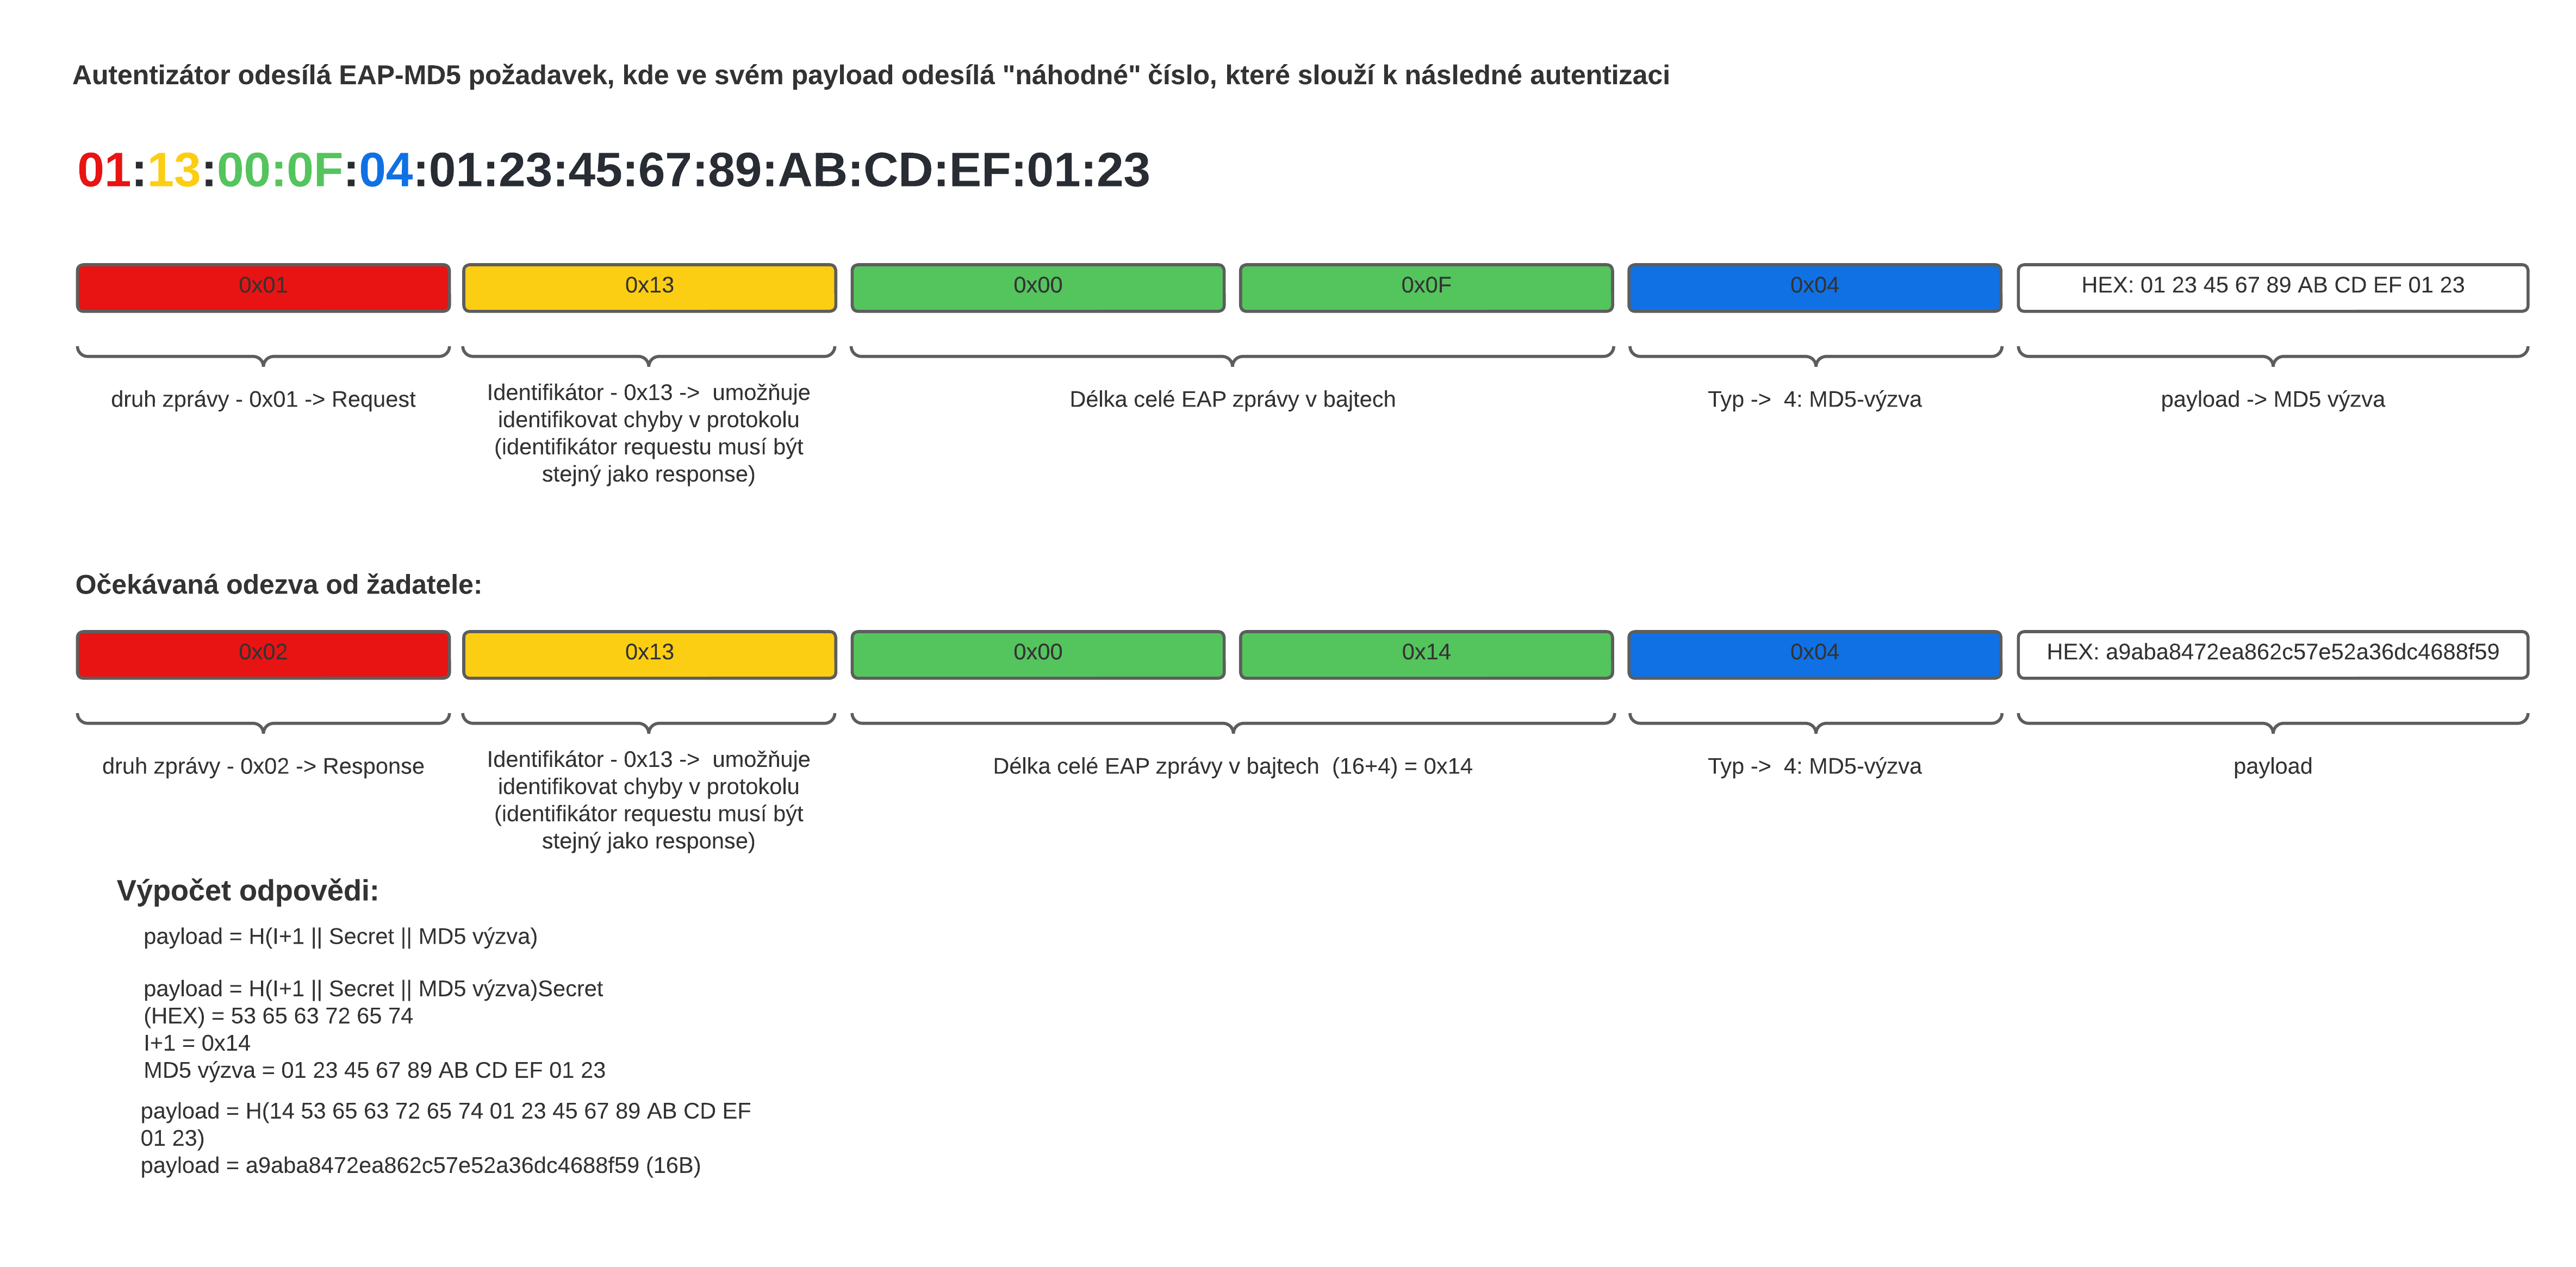
\includegraphics[width = 1\textwidth]{EAP.png}
			
		\end{figure}
		\section*{\large{\textbf{RADIUS}}}
		\item \textbf{Zadání:}\\
		
		Serveru byla z brány doručena následující zpráva protokolu RADIUS:\\
		01:02:00:22:00:11:22:33:44:55:55:77:88:99:AA:BB:CC:DD:EE:FF:01:07:4A:6F:73:65:66:
		02:07:F3:25:03:2A:BE.\\
		Víme přitom, že k zabezpečení provozu mezi branou a serverem je používán klíč K = Secret.
		U dané zprávy uveďte její typ a vysvětlete význam jednotlivých bajtů. Pokud se v ní vyskytuje
		přihlašovací jméno, tak je uveďte v textové podobě podle ASCII tabulky. Pokud se v ní bude
		nacházet zašifrované heslo, tak je dešifrujte a převeďte do textové podoby. Dále uveďte jaká bude
		odpověď serveru a význam jednotlivých bajtů této odpovědi vysvětlete. Předpokládejte přitom, že
		kontroly na straně serveru měly pozitivní výsledek.\\
		K výpočtu hešů a ke konverzi bajtů na text použijte stejné odkazy jako v předchozím příkladu
		\item \textbf{Vypracování:}\\

		\begin{figure}[ht!]
			\centering
			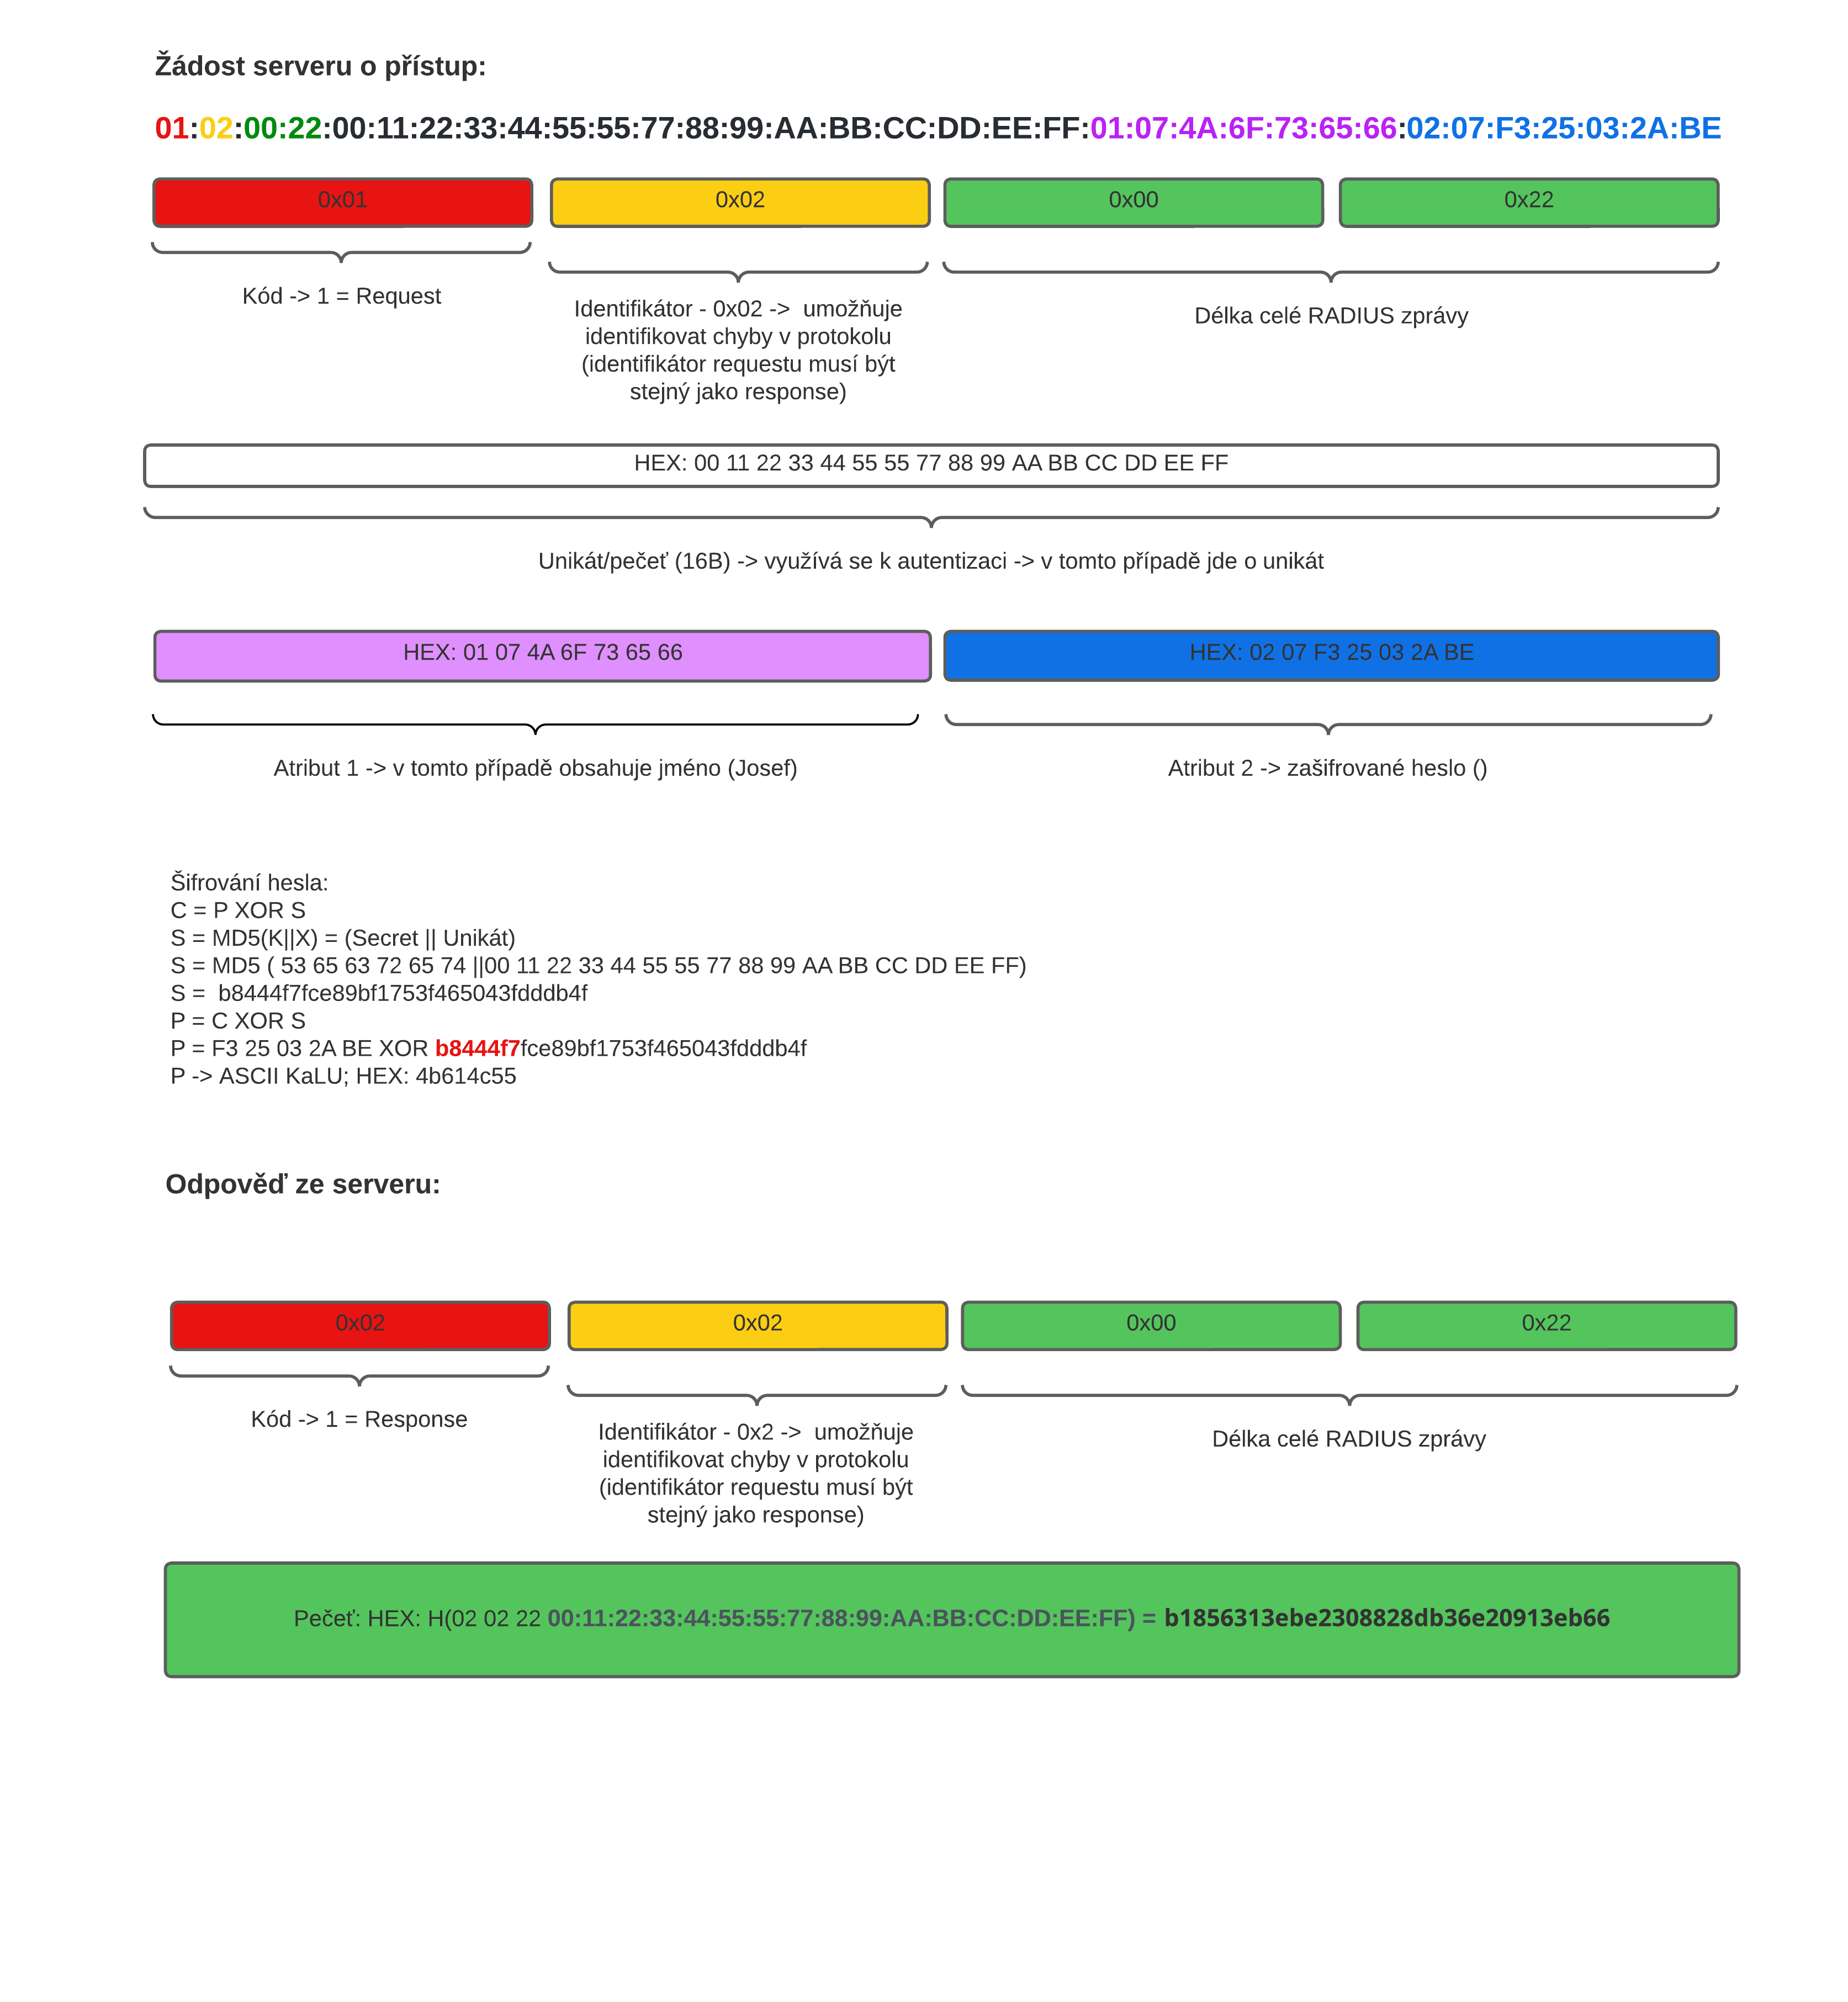
\includegraphics[width = 1\textwidth]{RADIUS.png}
			
		\end{figure}
	\end{itemize}

\end{document}
